\section{ParVSL}
I have forked the the original VSL project into a new language which I named Parallel VSL, or ParVSL.
ParVSL is fully backwards compatible with VSL and will be tested against it for performance.

VSL was a good candidate for this project because it featured a complete, working Lisp implementation while being
small enough to be a manageable project. The entire VSL codebase consists of around 10000 lines of code, all of which
was originally contained within a single file. Before making changes in critical areas, I spent some time familiarising
myself with the code. This included splitting the project in more more files, fixing a few obvious bugs, and porting
to C++.

\section{From C to C++}
The VSL language was written in the programming language C. C is a language with no standardised
multi-threaded model and no native support for multi-core programming. Furthermore, it has no well-defined
memory model, and no defined ordering of memory accesses. Multi-threaded programming
is only possible in C through a third-party library, such as \texttt{Windows threads} or the
the \texttt{POSIX threads} library on UNIX systems. Support further has to be guaranteed by individual compilers
and operating systems and can break between versions.

C++ is a superset of C and can compile existing, standard C code easily. The C++11 standard addresses the
above omissions, making C++ a multi-threaded language. While in some cases the implementation uses the same
libraries as the C equivalent (e.g POSIX), we do not have to think about these details and the code
we write is fully portable. The only requirement is that a C++11 compliant compiler is used and that it supports
the target platform. As of today, the C++11 standard has matured enough
that all the large compiler vendors (i.e GCC, Clang, Visual C++, Mingw, etc.) fully support it on the
major platforms (e.g x86, ARM and SPARC).

The first change I have made to the implementation is to clear it of any incompatible code and compile it
with a C++ compiler. This was a trivial task and mostly involved adding a few more explicit casts.
However, I have been slowly transitioning the code to idiomatic C++ as I analysed more parts of it
and became confident those changes wouldn't affect the semantics of the program.

\section{Throughput vs latency}
When optimising for performance in a programming language, we have to analyse the trade-off between
total throughput and latency. Optimising for latency means minimising the duration of any individual
task in the program, and increasing availability. Optimising for throughput involves minimising the
total running time of the program. For example, a web server would benefit more from reducing latency
of any individual request.

In a CAS program the user is most likely to care about throughput, i.e. compute the outputs of large
problem sizes as quickly as possible. The program is single-user and has a simple interface. The only case
for low latency is in the responsiveness of the graphical user interface. This is already provided by the
operating system so our main goal is directed towards minimising throughput in the application.
This is particularly important when designing the garbage collector.

\section{Memory allocation}
Memory is managed by the interpreter. It allocates a large block of memory at the beginning,
which it then manages as a contiguous array. When running out of memory, an extra block of the
same size as current available memory is malloc-ed, doubling the amount available. These blocks are
never freed until the end of the program. They are sorted by their pointer locations,
and carefully \emph{joined} together to maintain the abstract model of contiguous memory. Binary search
is used to identify the block containing a location.

% TODO: read-eval-print loop
% TODO: critical path

\begin{figure}[H]
    \centering
    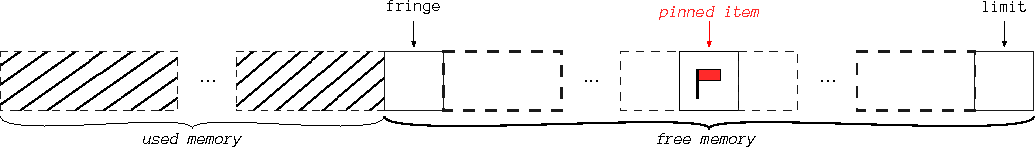
\includegraphics[width=1\linewidth]{vslalloc.pdf}
    \label{fig:vslalloc}
    \caption{Memory allocations in VSL}
\end{figure}

\section{Garbage collector}
An important feature of Lisp languages is the \emph{garbage collector}. Garbage collectors allow the programmer
to design code without having to worry about the lifecycle of their data, the internal memory model and
managing pointers. This makes Lisp code significantly easier to write, leaving the burden of providing safety and
efficiency to the compiler.

In effect, the garbage collector is an important component of the VSL interpreter and careful considerations
have to be made when modifying it. First of all, any bugs in the garbage collector may leave the memory in
an invalid state, corrupting the state of the program and leading to undefined behaviour in C. Such errors
are also very difficult to spot and debug, as they can go undetected until the particular region of memory
is accessed again. The original VSL memory allocation and garbage collector only supported a single-threaded model.

\subsection{Cheney's algorithm}
The approach a garbage collector uses to deal with freed memory affects both its performance and memory usage.
Before the first garbage collection cycle, memory can simply be allocated in a continuous fashion, making it
compact and fast. When the garbage collector finds unreachable objects and eliminates them, they will leave \emph{gaps} behind
and cause \emph{fragmentation}. Not dealing with fragmentation leads to wasted memory. Keeping track of the gaps
and filling them with objects of the right size involves extra book-keeping which can be quite expensive. Ultimately,
it is impossible to guarantee the gaps are filled efficiently, because the garbage collector cannot predict future
memory allocations, and thus heuristics have to be employed.

VSL avoids this problem entirely by using a \emph{copying} garbage collector. This means it compacts memory by moving
traceable objects to a new region. The unreachable objects are simply not moved and they will eventually be overwritten.
This method has the advantage that it fully compacts memory, fixing the issue of fragmentation in an efficient,
straight-forward way. The main trade-off is the total memory usage. A region of memory at least
as large as the one in use has to be used to copy the live objects into. In addition, when a very large amount
of memory is in use, the copying of all live memory might become more expensive than managing the free memory.
Finally, this approach is not incremental. The entire heap is scanned and cleaned every run. Other approaches might
reduce latency by collecting only partially in more, but shorter cycles.

The problem sizes in Reduce are usually not bound by memory on modern computers, with most of the test applications
using less than a gigabyte, although some users of Reduce elsewhere perform calculations
using tens or even hundreds of gigabytes elsewhere. Its application is also not latency-sensitive. It is used for
solving large problems as fast as possible. A large compaction stage is more efficient as it reduces time
switching between running code and collecting garbage and minimises fragmentation.
This makes the copying approach suitable for the language.

Cheney's algorithm \cite{cheney} is a method of \emph{stop-the-world} copying garbage collection.
The virtual \emph{heap} is divided into
two halves, and only one half is in use for allocations. The other half is considered free and used during garbage
collection. When the first half is full and garbage collection is triggered, all traceable objects are copied over
to the second half. Then, the two halves are swapped.

To start the tracing we need to consider a root set: a subset of object which are known to be accessible.
One example of elements in the root set is the table of symbols which are defined at the start
of the garbage collection. The stack will also contain pointers to objects and must be scanned when computing the root set.
While these are the main components of the root set, the interpreter may contain others depending on language features
and implementation, all of which must be spotted and added. The root set must be conservative as missing any object which
should be in the root set will result in collection of live objects, invalidating the program. It is always
preferable to over-approximate the root set.

Once we have distinguished a root set, we can trace all references to build the reachable set. Objects may contain references
to other objects, which are also considered reachable. For example, all elements of a list must be traced recursively.
The reachable set is the transitive closure of the reachability relation. All objects in the reachable set must be kept
during collection, while everything else may be safely collected.

The algorithm presented above is a heavily simplified abstraction. The root set includes other
locations apart from the symbol table, and all of them have to be handled carefully. This was an area
of particular importance when adding multi-threading.

The \texttt{copy} and \texttt{copycontent} procedures have to read the heap to determine the type, size and fields of
the \texttt{LispObject}, and act accordingly. This approach of storing all the information inside the virtual heap
and manually accessing it as needed has significant performance benefits. \texttt{LispObject} becomes a simple aliasing
for a pointer type, it allows many different types of objects (integers, floats, strings, lists) to be accessed
in a unified way, while staying compact in memory. The disadvantage is that it is is difficult to track memory
corruption, making debugging more difficult. This will become a problem if any bug in the code produces a data-race.

Please refer to appendix \ref{sec:cheneycode} for a more detailed implementation of the algorithm.

\subsection{Conservative GC}
One important design aspect of calculating the root set is how to handle references on the stack. Garbage collection
may start in the middle of a large computation and the references on the stack cannot be discarded. One safe, but slow
approach of dealing with this is to keep a virtual stack. Such a stack could be well typed and easily scanned to find
references. However, it would be much slower by adding a level of indirection to each expression, and it would also make
the code more difficult to manage.

Another approach is to tag words in memory. This approach is used, for instance, by the OCaml compiler, where the least
significant bit is a tag bit, indicating whether that word is a pointer reference or just data. This approach is better
than the virtual stack, but has the drawback of limiting the integer types (e.g 63bit vs 64), and requiring additional
instructions (i.e shifts) to do arithmetic.

The approach VSL uses is to be conservative. It treats all values on the stack as potential references, called \emph{ambiguous} roots.
This means we are overestimating the set of roots. Unlike \emph{unambiguous} roots (like the symbol table above), we
have to be careful when handling these values, and cannot manipulate them as \texttt{LispObject}. This rules out calling
\texttt{copy} or \texttt{copycontent} above on them, but they still need to be kept during garbage collection. The solution was
to \emph{pin} them. Any location on our heap which is pointed to by an ambiguous root is pinned and not copied over.
Additionally, the \texttt{allocate} function will have to check for pinned items on the heap and skip over them. This
additional book-keeping is manageable. When building the entirety of Reduce, the number of pinned items is never
larger than 300. Considering memory used is in the order of megabytes, these pinned locations cause negligible
fragmentation.

\section{Symbols and variable lifetime}
As the original language is decades old, its mechanism for variable lifecycle is not in line with that of modern languages.
This mechanism was counter-intuitive at first, and is lacking in providing safety to the user of the language.

There are two lifetime specifiers for symbols: \emph{global} and \emph{fluid}. It is important to note that they
do not refer semantically to variables but only to \textbf{symbol names}.

A \emph{global} symbol has only a single globally visible value. That means you cannot bind the name to any local
variable. For instance if \texttt{x} is declared global, it then cannot be used as a function parameter name, or in a
let binding.

A \emph{fluid} variable has a global value, but can also be locally bound. Fluids behave more like globals do
in other languages, allowing the name to be reused.

\texttt{Let} bindings and function parameters introduce \emph{local} symbols. If the symbol name is already declared global,
it will result in an error. If it is a fluid and has a global value, that value will be shadowed for the lifetime
of the binding.

To make it easier to use as a scripting language, Reduce's Lisp allows using symbols that aren't global, fluid,
or locally bound. These will act like local variables, except their lifetime will be defined for the duration of the
program. For single-threaded programs, this distinction is not important: these variables would act like fluids. However,
when implementing multithreading, fluids have a global value visible to all threads, while these symbols are only
visible on their local thread. I will call these symbols \emph{unbound locals}.

\section{Saving state to disk}
Reduce has an important feature which allows the user to preserve the state to disk. A \texttt{preserve} instruction can be
used to do so, and the user is able to specify a function to run on restart. Preserve saves the entire state of the
program, including memory and symbols. The feature involves careful manipulation of the world state and keeping it
unaffected when enabling multi-threaded programs is complicated. I ran into a few challenges when implementing ParVSL,
which I will discuss in the implementation section.
